\documentclass{article}
\usepackage{graphicx,fancyhdr,amsmath,amssymb,amsthm,subfig,url,hyperref,enumerate,tkz-berge}
\usepackage[margin=1in]{geometry}

%----------------------- Macros and Definitions --------------------------

%%% FILL THIS OUT
\newcommand{\studentname}{Keyan Pishdadian}
\newcommand{\uwid}{keyanp}
\newcommand{\exerciseset}{Exercise Set 1}
%%% END



\renewcommand{\theenumi}{\bf \Alph{enumi}}

%\theoremstyle{plain}
%\newtheorem{theorem}{Theorem}
%\newtheorem{lemma}[theorem]{Lemma}

\fancypagestyle{plain}{}
\pagestyle{fancy}
\fancyhf{}
\fancyhead[RO,LE]{\sffamily\bfseries\large University of Washington}
\fancyhead[LO,RE]{\sffamily\bfseries\large  Incentives in Computer Science}
\fancyfoot[LO,RE]{\sffamily\bfseries\large \studentname: \uwid @uw.edu}
\fancyfoot[RO,LE]{\sffamily\bfseries\thepage}
\renewcommand{\headrulewidth}{1pt}
\renewcommand{\footrulewidth}{1pt}

\graphicspath{{figures/}}

%-------------------------------- Title ----------------------------------

\title{\textbf{Solutions to \exerciseset}}
\author{\studentname \qquad Student ID: \uwid}

%--------------------------------- Text ----------------------------------

\begin{document}
\maketitle

\section*{Notation}
Throughout this document, $s_{x,y}^x$ represents an agent $s$ initially assigned $x$, with the preference order $x, y$. If there is no initial assignment then only preference order is shown, i.e. $s_{x,y}$.

\section*{Exercise 1}
\begin{enumerate}[a.]
\item %a
\textit{Claim.} Serial dictatorship is group-strategyproof.

\begin{proof} Let $U$ be the set of all students. Let $S \subseteq U$. $\forall S \in U$, let $i$ be the first student to be considered in $S$. When $i$ is considered, they can do no better than their top preference at that point, so being truthful is the dominant strategy. The same then holds for each subsequently considered student in $S$.
\end{proof}

\item %b
The error is in the line "Now, since telling the truth is a dominant strategy, it can’t be the case that someone who told the truth got a worse outcome in $O_L$ than in $O_T$". This is because the property of a mechanism being truthful means that honesty is the best policy when agents act alone, it does not make it impossible that "that someone who told the truth got a worse outcome in $O_L$ than in $O_T$". That statement is only true if the mechanism is also group-strategyproof.

\item %c

Let there be 4 students: $A, B, C, D$, and 4 offices: $1, 2, 3, 4$. \newline
Let the preferences and initial assignments of the students be: $A_{2,3,1,4}^1, B_{3,1,2,4}^2, C_{1,2,3,4}^3, D_{1,2,3,4}^4$ and the order for step 2: $D, C, A, B$. The resulting assignments under serial dictatorship would be: $A_{3}, B_{4}, C_{2}, D_{1}$. With only $D$ getting their top choice office.

This is unstable because students $A^1, B^2, C^3$ are incentivized to refuse participation and swap their initially assigned offices, resulting in the assignments: $A_{2}, B_{3}, C_{1}, D_{4}$. With all of $A, B, C$ strictly better off and with their top choice.

\end{enumerate}

\section*{Exercise 2}
This mechanism is not strategyproof. If a student's list includes popular schools then they are more likely to not match and be skipped during a phase (step 3). So agents are incentivized to be untruthful about their preferences and select less popular/sought-after schools in order to maximize their chances at matching in an early phase. As with any non-strategyproof mechanism, lack of information and/or sophistication is a disadvantage in this mechanism as well. Because of this I would assume that lower income and less educated parents and their students (children) would be harmed more as they would be less likely to be aware of how to produce a successful strategy.

\section*{Exercise 3}
\textit{Claim.} Every stable matching is also Pareto optimal.
\begin{proof}
For the sake of contradiction, let $M$ be a matching which is stable but not Pareto optimal, so there also be another matching $M'$ in which at least one agent does better and none does worse.\\ \\
Let this agent be $h$ and $(h, s) \in M$ is the pair matching $h$ and $s$. By definition there must be another pair $(h, s') \in M'$ in which $h$ prefers $s'$ to $s$. Because all preferences are strict and $s'$ cannot be worse off, then $s'$ must prefer their current match $(h, s') \in M'$ to their prior match $(h', s') \in M$.\\ \\
It follows that $h$ ranks $s'$ higher than $s$, and $s'$ ranks $h$ higher than $h'$\\ \\
$\therefore$ $(h, s') \in M$ form a blocking pair and $M$ cannot be a stable matching, a contradiction.
\end{proof}
\section*{Exercise 4}
\textit{Claim.} Not every Pareto optimal matching is also stable.
\begin{proof}
By counterexample. Let there be a matching $M$:
\[
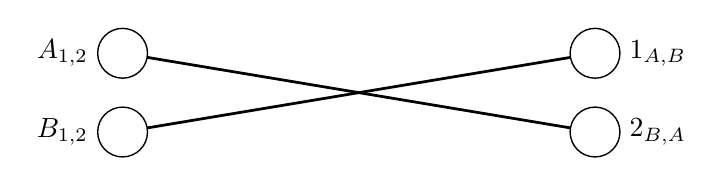
\begin{tikzpicture}[every fit/.style={draw,inner sep=-2pt,text width=2cm, line width=pt}]
\GraphInit[vstyle=Normal]
    \SetUpVertex[Math,Lpos=-180,LabelOut]
    \Vertex[x=0,y=1,LabelOut=true]{A_{1,2}}
    \Vertex[x=0,y=0,LabelOut=true]{B_{1,2}}
    \SetUpVertex[Lpos=0]
    \Vertex[x=6,y=1,LabelOut=true]{1_{A,B}}
    \Vertex[x=6,y=0,LabelOut=true]{2_{B,A}}
    \SetUpEdge[lw=1pt,color=black]
    \Edges(A_{1,2}, 2_{B,A})
    \Edges(B_{1,2}, 1_{A,B})
\end{tikzpicture}\\
\]
The only alternative matching has $A, 1, 2$ all doing strictly better but $B$ doing strictly worse, so $M$ is Pareto optimal. However, $M$ is not stable because $(A, 1)$ form a blocking pair who both prefer each other to their match in $M$.
\end{proof}

\section*{Exercise 5a}
\begin{enumerate}[i.]

\item %i
\textit{Claim.} Serial dictatorship always outputs a Pareto optimal matching.
\begin{proof}
Let $M$ be a matching outcome of the serial dictatorship mechanism. Let $s_i$ and $u_i$ be the student and university matched in round $i$, respectively.\\ \\
When $s_i$ is considered, she can only select from $\{u_{i}, ..., u_n\}$, from which she receives her top choice $u_i$. If $s_i$ is matched to any other $u \in \{u_{i}, ..., u_n\}$ she will do worse, and the only way she could do better is to match with some $u \in \{u_{1}, ..., u_{i-1}\}$. But given that $s_1, ..., s_{i-1}$ received their top choice remaining when they were considered, matching $s_i$ with some $u \in \{u_{1}, ..., u_{i-1}\}$ would make some $s \in \{s_1, ..., s_{i-1}\}$ strictly worse off. Therefore $M$ is Pareto optimal.
\end{proof}

\item %ii
\textit{Claim.} Serial dictatorship does not always outputs a stable matching.
\begin{proof}
By counterexample. Let there be two students $A, B$, the consideration order for serial dictatorship be: $A, B$, and the student preferences given below. The outcome of the serial dictatorship mechanism is the matching $M$:
\[
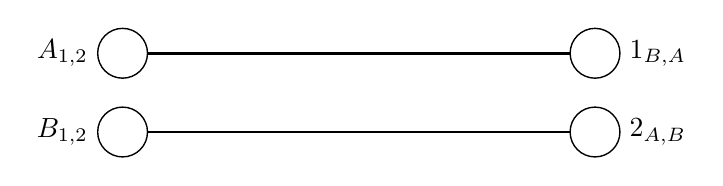
\begin{tikzpicture}[every fit/.style={draw,inner sep=-2pt,text width=2cm, line width=pt}]
\GraphInit[vstyle=Normal]
    \SetUpVertex[Math,Lpos=-180,LabelOut]
    \Vertex[x=0,y=2,LabelOut=true]{A_{1,2}}
    \Vertex[x=0,y=1,LabelOut=true]{B_{1,2}}
    \SetUpVertex[Lpos=0]
    \Vertex[x=6,y=2,LabelOut=true]{1_{B,A}}
    \Vertex[x=6,y=1,LabelOut=true]{2_{A,B}}
    \SetUpEdge[lw=1pt,color=black]
    \Edges(A_{1,2}, 1_{B,A})
    \Edges(B_{1,2}, 2_{A,B})
\end{tikzpicture}
\]
In this matching $B$ prefers $1$ over $2$, and $1$ prefers $B$ over $A$, there fore $(B, 1)$ are a blocking pair and $M$ is not stable.
\end{proof}

\item %iii
\textit{Claim.} In this mechanism it is in each student's best interest to report their preferences truthfully.
\begin{proof}
Let $s_i$ and $u_i$ be the student and university matched in round $i$, respectively. When $s_i$ is being considered she cannot match to any $u \in \{u_{1}, ..., u_{i-1}\}$, her best match must be her true most preferred university $u \in \{u_{i}, ..., u_n\}$.
\end{proof}

\item
\textit{Claim.} In this mechanism it is in each university's best interest to report their preferences truthfully.
\begin{proof}
Universities' preferences are not considered in this mechanism, so their reported preferences do not change the outcome of the mechanism. Therefore, truthfulness is at least as good as any other strategy.
\end{proof}
\end{enumerate}

\section*{Exercise 5b}
\begin{enumerate}[i.]

\item %i
\textit{Claim.} Weighted matching always outputs a Pareto optimal matching.
\begin{proof}
For the sake of contradiction, let $M$ be a non-Pareto optimal minimum-weight perfect matching outcome from a run of the weighted matching mechanism. By definition of Pareto optimality, there must exist another matching $M'$ in which one agent is doing better and the rest are doing at least as well as in $M$. Let $\vec{w}$ and $\vec{w'}$ be the sum of edge weights in $M$ and $M'$, respectively.\\
\\
By design of the mechanism we know that if one agent is doing better in $M'$ and none are doing worse then $\vec{w} > \vec{w'}$. But if $\vec{w} > \vec{w'}$ then $M$ was not the minimum-weight perfect matching as there exists another matching with lower total edge weight, a contradiction.
\end{proof}

\item
\textit{Claim.} Weighted matching does not always output a stable matching.
\begin{proof}
By counterexample. Consider the agent preferences resulting in the following weighted graph created using the mechanism:
\[
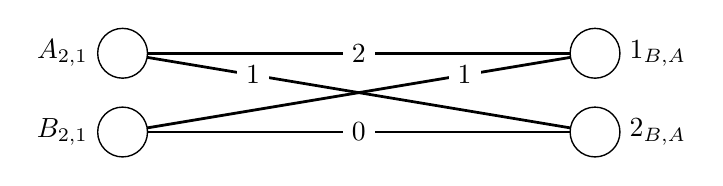
\begin{tikzpicture}[every fit/.style={draw,inner sep=-2pt,text width=2cm, line width=pt}]
\GraphInit[vstyle=Normal]
    \SetUpVertex[Math,Lpos=-180,LabelOut]
    \Vertex[x=0,y=2,LabelOut=true]{A_{2,1}}
    \Vertex[x=0,y=1,LabelOut=true]{B_{2,1}}
    \SetUpVertex[Lpos=0]
    \Vertex[x=6,y=2,LabelOut=true]{1_{B,A}}
    \Vertex[x=6,y=1,LabelOut=true]{2_{B,A}}
    \SetUpEdge[lw=1pt,color=black]
    \Edge[label=$2$](A_{2,1})(1_{B,A})
    \Edge[label=$1$,style={pos=0.25}](A_{2,1})(2_{B,A})
    \Edge[label=$1$,style={pos=0.75}](B_{2,1})(1_{B,A})
    \Edge[label=$0$](B_{2,1})(2_{B,A})
\end{tikzpicture}
\]
Both possible matchings have the same total edge weight, so lexicographical tie-breaking results in the matching $M$:
\[
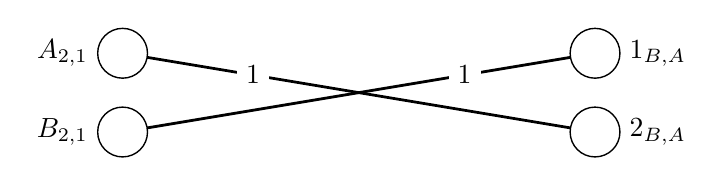
\begin{tikzpicture}[every fit/.style={draw,inner sep=-2pt,text width=2cm, line width=pt}]
\GraphInit[vstyle=Normal]
    \SetUpVertex[Math,Lpos=-180,LabelOut]
    \Vertex[x=0,y=2,LabelOut=true]{A_{2,1}}
    \Vertex[x=0,y=1,LabelOut=true]{B_{2,1}}
    \SetUpVertex[Lpos=0]
    \Vertex[x=6,y=2,LabelOut=true]{1_{B,A}}
    \Vertex[x=6,y=1,LabelOut=true]{2_{B,A}}
    \SetUpEdge[lw=1pt,color=black]
    \Edge[label=$1$,style={pos=0.25}](A_{2,1})(2_{B,A})
    \Edge[label=$1$,style={pos=0.75}](B_{2,1})(1_{B,A})
\end{tikzpicture}
\]
Where $(B, 2) \in M$ form a blocking pair, therefore $M$ is not a stable matching.
\end{proof}

\item %iii
\textit{Claim.} In this mechanism it is not always in each student's best interest to report their preferences truthfully.
\begin{proof}
By counterexample. Let there be three students $A, B, C$ and three universities $1, 2, 3$ with their preferences given below. The weighted graph created by this mechanism (omitted for simplicity) has a minimum-weight matching of 6, with many possible matchings giving this weight. Lexicographical tie-breaking gives the matching $M$:
\begin{equation}
\label{eqn:truth}
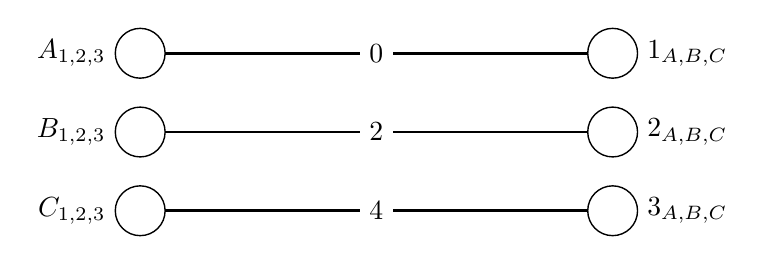
\begin{tikzpicture}[every fit/.style={draw,inner sep=-2pt,text width=2cm, line width=pt}]
\GraphInit[vstyle=Normal]
    \SetUpVertex[Math,Lpos=-180,LabelOut]
    \Vertex[x=0,y=2,LabelOut=true]{A_{1,2,3}}
    \Vertex[x=0,y=1,LabelOut=true]{B_{1,2,3}}
    \Vertex[x=0,y=0,LabelOut=true]{C_{1,2,3}}
    \SetUpVertex[Lpos=0]
    \Vertex[x=6,y=2,LabelOut=true]{1_{A,B,C}}
    \Vertex[x=6,y=1,LabelOut=true]{2_{A,B,C}}
    \Vertex[x=6,y=0,LabelOut=true]{3_{A,B,C}}
    \SetUpEdge[lw=1pt,color=black]
    \Edge[label=$0$,style={pos=0.5}](A_{1,2,3})(1_{A,B,C})
    \Edge[label=$2$,style={pos=0.5}](B_{1,2,3})(2_{A,B,C})
    \Edge[label=$4$,style={pos=0.5}](C_{1,2,3})(3_{A,B,C})
\end{tikzpicture}
\end{equation}
Although $C$ has a true preference of $C_{1,2,3}$, lying and recording the preference $C_{2,1,3}$ results in a more optimal minimum-weight matching of 5 and gives $C$ her true second choice university rather than her true third choice.
\[
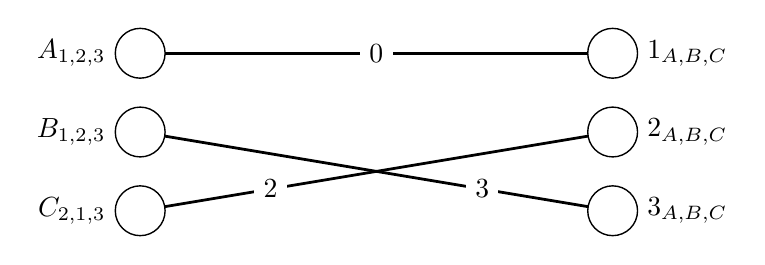
\begin{tikzpicture}[every fit/.style={draw,inner sep=-2pt,text width=2cm, line width=pt}]
\GraphInit[vstyle=Normal]
    \SetUpVertex[Math,Lpos=-180,LabelOut]
    \Vertex[x=0,y=2,LabelOut=true]{A_{1,2,3}}
    \Vertex[x=0,y=1,LabelOut=true]{B_{1,2,3}}
    \Vertex[x=0,y=0,LabelOut=true]{C_{2,1,3}}
    \SetUpVertex[Lpos=0]
    \Vertex[x=6,y=2,LabelOut=true]{1_{A,B,C}}
    \Vertex[x=6,y=1,LabelOut=true]{2_{A,B,C}}
    \Vertex[x=6,y=0,LabelOut=true]{3_{A,B,C}}
    \SetUpEdge[lw=1pt,color=black]
    \Edge[label=$0$,style={pos=0.5}](A_{1,2,3})(1_{A,B,C})
    \Edge[label=$3$,style={pos=0.75}](B_{1,2,3})(3_{A,B,C})
    \Edge[label=$2$,style={pos=0.25}](C_{2,1,3})(2_{A,B,C})
\end{tikzpicture}
\]
\end{proof}

\item %iv
In this mechanism there is no difference in treatment between students and universities so similar to (iii) it is not always in a universities' best interest to be truthful. If we consider the matching provided earlier \eqref{eqn:truth}, if the university $3$ lies and records the preference $3_{B,A,C}$ then a more optimal minimum-weight matching of 5 is possible and gives $3$ its true second choice student rather than its true third choice.
\[
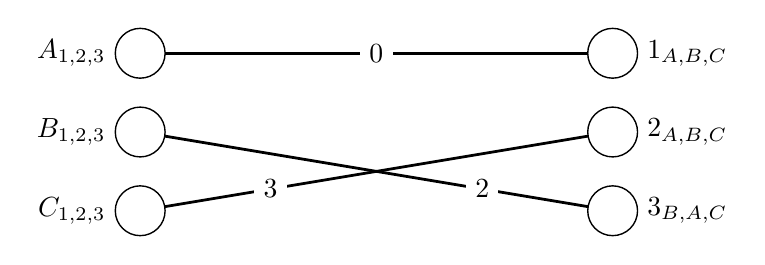
\begin{tikzpicture}[every fit/.style={draw,inner sep=-2pt,text width=2cm, line width=pt}]
\GraphInit[vstyle=Normal]
    \SetUpVertex[Math,Lpos=-180,LabelOut]
    \Vertex[x=0,y=2,LabelOut=true]{A_{1,2,3}}
    \Vertex[x=0,y=1,LabelOut=true]{B_{1,2,3}}
    \Vertex[x=0,y=0,LabelOut=true]{C_{1,2,3}}
    \SetUpVertex[Lpos=0]
    \Vertex[x=6,y=2,LabelOut=true]{1_{A,B,C}}
    \Vertex[x=6,y=1,LabelOut=true]{2_{A,B,C}}
    \Vertex[x=6,y=0,LabelOut=true]{3_{B,A,C}}
    \SetUpEdge[lw=1pt,color=black]
    \Edge[label=$0$,style={pos=0.5}](A_{1,2,3})(1_{A,B,C})
    \Edge[label=$2$,style={pos=0.75}](B_{1,2,3})(3_{B,A,C})
    \Edge[label=$3$,style={pos=0.25}](C_{1,2,3})(2_{A,B,C})
\end{tikzpicture}
\]
\end{enumerate}

\end{document}
